\documentclass[a4paper,10pt,openright,openbib,twocolumn]{article}
%\usepackage[portuges]{babel}
\usepackage[T1]{fontenc}
\usepackage{ae}
\usepackage[utf8]{inputenc}
\usepackage[pdftex]{graphicx}
\usepackage{url}
\usepackage{listings}
\usepackage{verbatim}
\usepackage{enumerate}
\usepackage[pdftex, bookmarks, colorlinks, linkcolor=black, urlcolor=blue]{hyperref} 
\usepackage[a4paper,left=2.5cm,right=2.5cm,top=3.5cm,bottom=3.5cm]{geometry}
\usepackage{colortbl}
\usepackage[margin=10pt,font=small,labelfont=bf]{caption}
\usepackage{mdwlist}
\usepackage{cleveref}
\usepackage{epsfig}

\usepackage{multicol}
\usepackage{appendix}
\usepackage{float}

\setlength{\parindent}{0cm}
\setlength{\parskip}{2pt}


\begin{document}

\begin{multicols}{2}
\title{Study and Optimization of a Finite Volume Application}
\author{
    Brito, Rui\\
    PG22781\\
    Department of Informatics\\
    University of Minho\\
    ruibrito666@gmail.com
  \and
    Alves, José\\
    PG22765\\
    Department of Informatics\\
    University of Minho\\
    zealves.080@gmail.com
}
\date{}
\maketitle
\end{multicols}

\section{Introduction}

This study presents an analysis of the application conv-diff. This analysis consists in the application profile, the use of several optimization techniques and the discussion of its results.
The program conv-diff calculates the heat transfer through an area using a Finite Volume method.

The goal of this study is to research different optimization techniques and to achieve an improvement in the application performance.

The study was divided in several stages.
In the first stage a profile of the application was created, identifying its troublesome areas and improving the sequential version.
A second stage dedicated to a shared-memory version using OpenMP.
The third stage to work with a GPU version, using its massive parallelism capabilities, was made in CUDA.
In the fourth stage a naive distributed-memory version was researched using MPI.
Finally in the fifth and final stage one technique of the previous stages was chosen and improved upon. Based on our previous results, the progression to an improved OpenMP version seemed obvious and was pursued.


In section \ref{case}, we presented the problem at hand along with its mathematical formulation. In section \ref{testmet} we present the test methodology and the machines used all throughout the project. Section \ref{naive} presents the first steps we took with conv-diff, which is to say, the first optimizations we did. Section \ref{openmp} shows the OpenMP implementation along with some results. In section \ref{mpi} we can see the details of our mpi implementation, while section \ref{final} provides some insight into our final implementation of the problem. Section \ref{conc} provides some concluding remarks. 

\section{Case Study}
\label{case}
The application analyzed for this study is \emph{conv-diff(Convection-Diffusion)}.This application simulates the way heat is transferred in a fluid using the finite-volumes method.To compute the heat diffusion, the surface is represented as a mesh. Being represented by cells and edges, the algorithm will traverse all edges, calculating the contribution of the adjacent cells. This application rests in a Finite Volume Library (FVLib), which handles the structures and some of the logic functions necessary for the problem's solution.

The application's main objective is to compute a vector $\overline{\phi}$ such that $\overline{\phi} \longrightarrow G(\overline{\phi}) = \left(\begin{array}{c}
0\\
0\\
\vdots\end{array}\right)$
This is accomplished in three different stages:
\begin{enumerate}
    \item {We begin with a candidate vector $\phi$}
    \item {For each edge, we compute the flux $F_{ij}$, with $i$ and $j$ being the indexes of the adjacent cells}
    \item {For each cell, we compute $\sum |e_{ij}| F_{ij} - |c_i| f_i$}
\end{enumerate}
Thus: $\phi = \left(\begin{array}{c}
\phi_1\\
\vdots\\
\phi_I
\end{array}\right) \longrightarrow G = \left(\begin{array}{c}
G_1\\
\vdots\\
G_I
\end{array}\right)$


The output can be converted to msh format, which is compatible with gmsh, for following data visualization(\cref{fig:parallel}).

\begin{figure}[!htb]
    \centering
    \begin{minipage}[t]{\columnwidth}
        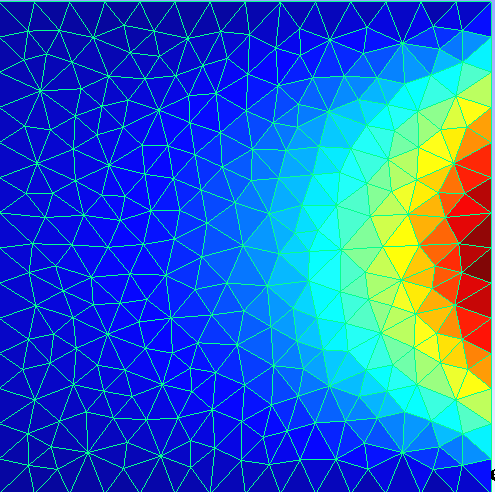
\includegraphics[width=\textwidth]{../images/mesh_output.png}
        \caption{Output example.\label{fig:parallel}}
    \end{minipage}
\end{figure}

\section{Test Methodology}
\label{testmet}

In order to achieve precise and consistent results, all tests were run on a dedicated execution of the algorithm, with niceness set to -20, to ensure the tests execution was top priority to the OS's scheduler. Furthermore, all network connections were disabled. To decrease the chance of human error, all tests were hard-coded into a bash script, with another script traversing those tests and showing the results. Also, it should be noted that every test was run at least 3 times. A 5\% error margin was checked between execution (the aforementioned script handles this part), and if this margin is not met, the tests are run again. \\

The table below describes all the machines used throughout this project. The most used machines are the MacBookPro and compute-601@search.

\begin{center}

            \begin{table}[!htb]
            \resizebox{\columnwidth}{!}{
            \begin{tabular}{|c|c|c|c|c|}
            \hline
             & compute-511@search & compute-601@search & compute-101@search & MacBookPro\\
             & AMD Opt 6174 & Xeon X5650 & Xeon E7520 & Intel Ivy-Bridge i7\\
            \hline
            \# processors & 2 & 2 & 2 & 1\\
            \# cores per processor & 12 & 6 & 1 & 4\\
            hyper-threading & - & yes & yes & yes\\
            clock frequency(G!htbz) & 2.2 & 2.66 & 3.2 & 2.3\\
            L1 capacity & 128KB & 32KB & 16KB & 64KB\\
            L2 capacity & 512KB & 256KB & 2MB & 256KB\\
            L3 capacity & 12MB & 12MB & - &6MB\\
            RAM capacity & 64GB & 48GB & 2GB & 16GB\\
            \hline
            \end{tabular}}
            \caption{Test machines}         
            \end{table}
        \end{center}

\section{Na\"{i}ve Optimization}
\label{naive}

The program consists of four major parts, reading the initial mesh from a file. Then, using the functions \emph{makeResidual}, which calls the function \emph{makeFlux}, the flux contributions are calculated and the vector phi is built, thus achieving a matrix free implementation. Following this, to calculate the deviation in the results from the previous operations, the function \emph{LUFactorize}. Finally, both the meshes are written to the output files, together with the error between them.
 
After analyzing the application, we conclude that the algorithm has a very high workload in the \emph{LUFactorize} function, comprising of more than 90\% of the execution time.
This is mostly because LUFactorize is a matrix implementation of the algorithm presented in the previous section. While it provides accurate results, its memory usage, for example, makes it unusable for big meshes. As an example, a mesh with more than fifty thousand cells will easily consume more than 10 GB of RAM.

After dissecting the code and understanding the problem at hand, we began to notice several implementation errors, these errors, such as reading the same variable repeatedly from a file and long chains of calculation with a heavy division at the end, were easy to spot, and could clearly been avoided. We changed all those trivial aspects of the application, which required minimal effort. That being said, this simple optimizations paid results. The computation time has been greatly reduced, with the aforementioned \emph{LUFactorize} function taking an even more prominent role in our profile. Since \emph{LUFactorize} is very time-consuming and could overshadow the part of the program we were focusing on, we removed it.

Below is table of results we got from PAPI, displaying the difference between the original version and the best sequential version. 
These results show the improvements our small changes got. By not computing the same value in every iteration of the loop and making those values constant, we greatly reduced the number of loads and stores and, consequently, the number of cache accesses. This is because the \emph{const} keyword tells the compiler that a particular variable will not change during runtime.  

\begin{table}[!htb]
    \resizebox{\columnwidth}{!}{
        \begin{tabular}{|c|c|c|}
        \hline
            & original version & optimized sequential version\\
        \hline
            Total instructions & 2.517.584 & 285.551\\
            Load instructions & 630.156 & 86.532\\
            Store instructions & 326.459 & 39.208\\
            FP operations & 55.673 & 44.019\\
            L1 data accesses & 1.061.761 & 153.593\\
            L2 data accesses & 22.914 & 17.467\\
        \hline
        \end{tabular}}
    \caption{PAPI comparison}
    \label{tab:testcases}
\end{table}

\section{Shared Memory Parallel Optimization(OpenMP)}
\label{openmp}

After optimizing the sequential code, we turned our efforts to parallelizing the code. The two loops responsible for the matrix free calculations were ideal candidates. We parallelized both this loops. We had some struggles with data-races in these, but we overcame the problems rather easily. The data-races exist because the mesh is traversed by the edges, however, as we found out, if they are traversed by cell, these data-races no longer exist. Also, the library that was provided includes some iterator style structures. These were also a problem, because, while OpenMP as no problem in parallelizing STL iterators, this doesn't hold for \emph{FVlib}'s iterators. So, we had to convert those to a standard for loop. The code was successfully parallelized, however, results were disappointing, execution time didn't decrease at all, hinting at a memory bound application.

Below is a graph detailing the results we got for the parallel portion of the program. We ran this test on an Intel Xeon 5650, which has 12 physical cores and hyperThreading. As this processor has 12 cores it got us wondering if it would scale any better in a processor with 24 physical cores, so we also ran the tests on an AMD Opteron 6174. Also, as most of the optimizations were made in a personal machine, we included those results as well. The faster times can be explained the the use of a recent compiler. The processor is an Intel Ivy Bridge i7 (2.3 Ghz) with 4 physical cores. The slower times on the AMD machine can be explained by bad space locality. One of the strengths of the AMD processor is it's big cache, however, logically, if the program as bad locality, it will perform worse than in it's Intel counterpart. 
As it can be seen, the application doesn't scale at all as expected, this is because of the high number of memory accesses. Also, the deep indirection chain in \emph{FVLib} plays it's part, with every structure being a collection of pointers to other structures.

\begin{figure}[!htb]
    \centering
    \begin{minipage}[t]{\columnwidth}
        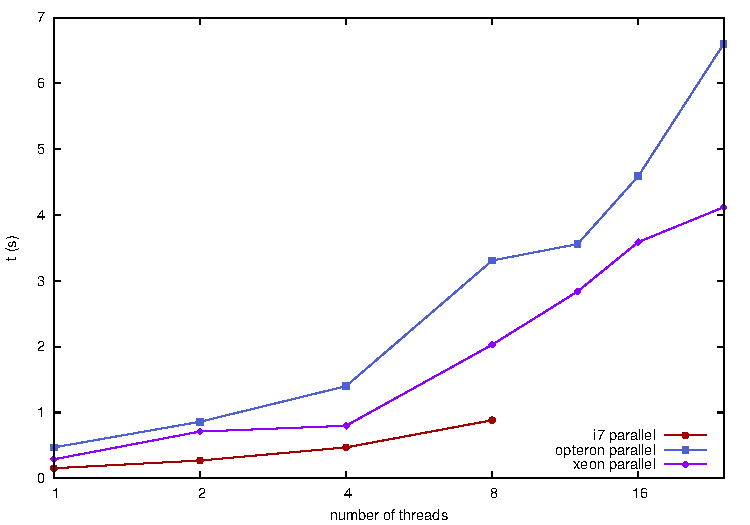
\includegraphics[width=\textwidth]{../../../openmp/results/parallel.pdf}
        \caption{Scalability of the parallel region \label{fig:parallel}}
    \end{minipage}
\end{figure}

Figure \ref{fig:total} is a plot of the total execution times.

\begin{figure}[!htb]
    \centering
    \begin{minipage}[t]{\columnwidth}
        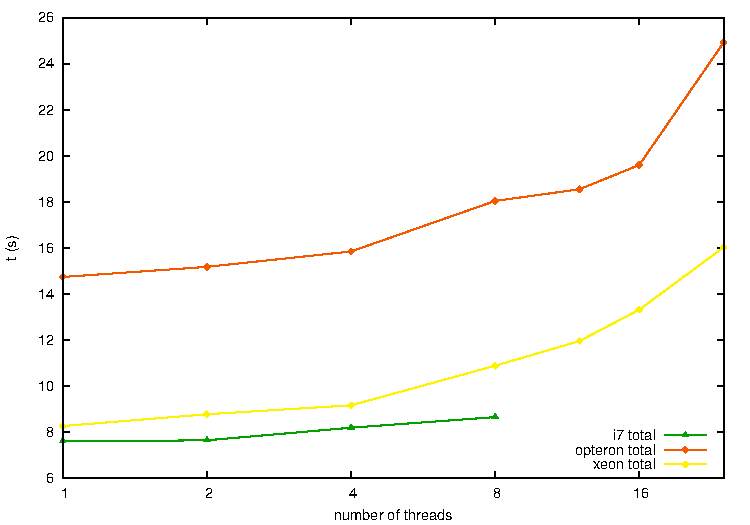
\includegraphics[width=\textwidth]{../../../openmp/results/total.pdf}
        \caption{Total execution time \label{fig:total}}
    \end{minipage}
\end{figure}

\section{Distributed Memory Optimization(MPI)}
\label{mpi}

Another approach we tried for optimizing the code was an MPI version. The strategy was to have a master process coordinating some slave processes. Each slave process computed a pre-assigned part of the mesh, an then, the results were colected by the master thread. Below is an illustration of what would typically happen.

\begin{figure}[!htb]
    \centering
    \begin{minipage}[t]{\columnwidth}
        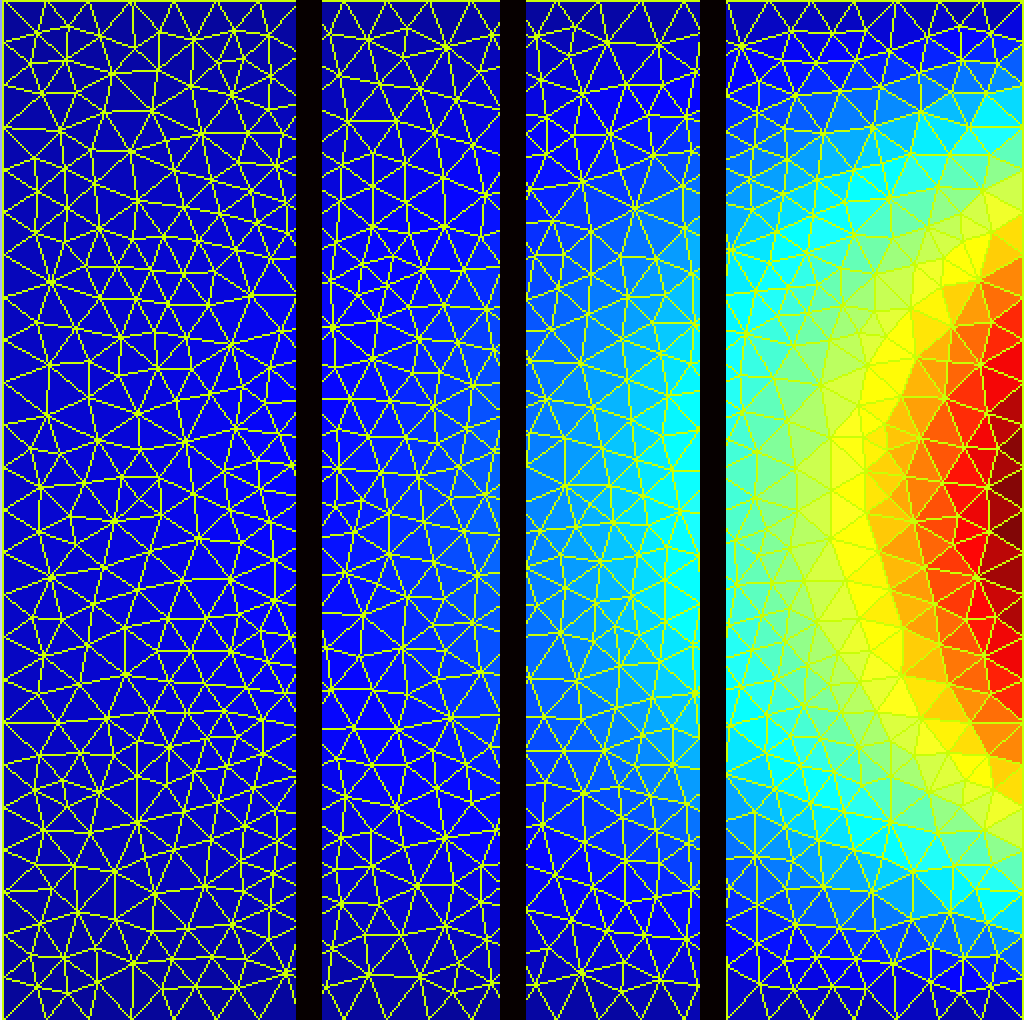
\includegraphics[width=\textwidth]{../images/mesh_vertical.png}
        \caption{Total execution time \label{fig:mes_vert}}
    \end{minipage}
\end{figure}

Figure \ref{fig:mes_vert} shows the way we partitioned the mesh, which is, at best, problematic. Since the fluxes are computed from right to left, one can easily see the high level of barrier synchronization and communication needed where the mesh was partitioned. Another problem with this implementation is because of the way the mesh is stored. Since we don't know where a particular cell is, another level of synchronization arises, because we can't compute the flux of a cell in a section, before the previous section is computed. 
Some of FVLib's templates were hard to serialize and some balancing problems were also encountered. This version proved to be very problematic, causing some error spikes, almost the final result.

Below are two plots portraying both the speedups achieved and the communication rate. 

\begin{figure}[!htb]
    \centering
    \begin{minipage}[t]{\columnwidth}
        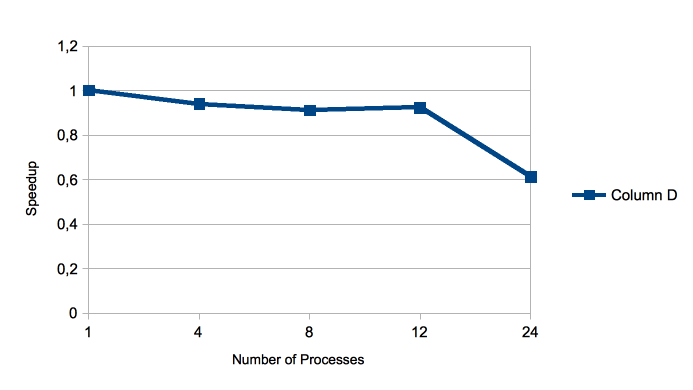
\includegraphics[width=\textwidth]{../../../mpi/slides/images/speedup.png}
        \caption{Speedups\label{fig:speedmpi}}
    \end{minipage}
\end{figure}

\begin{figure}[!htb]
    \centering
    \begin{minipage}[t]{\columnwidth}
        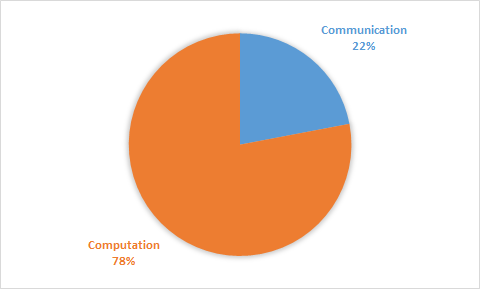
\includegraphics[width=\textwidth]{../../../mpi/slides/images/com.png}
        \caption{Communication share \label{fig:com}}
    \end{minipage}
\end{figure}

As it can be on figure \ref{fig:com}, a real speedup was never achieved, despite the fact that it does scale from 8 to 12 processes. With 24, it's already too many, and communication costs make this implementation inviable. The communication share can be seen in figure \ref{fig:speedmpi}


\section{Final Implementation}
\label{final}

In this final implementation, we opted to make our shared memory implementation better. To achieve this, we started by trying to solve all the problems that have plaguing us since the beggining. We converted the necessary structures to SOA, however, because of the way the mesh read from a file, we weren't able to solve the mesh locality problem, altghout its effects were softened. The main problem with the mesh is that \emph{gmsh} does not optimize the mesh structure. We could sort the mesh before it is used, however, a tight schedule prevented us from doing so. Also, it could have a bad impact on performance. 

The results we got are displayed below. 

    \begin{figure}[H]
        \centering   
        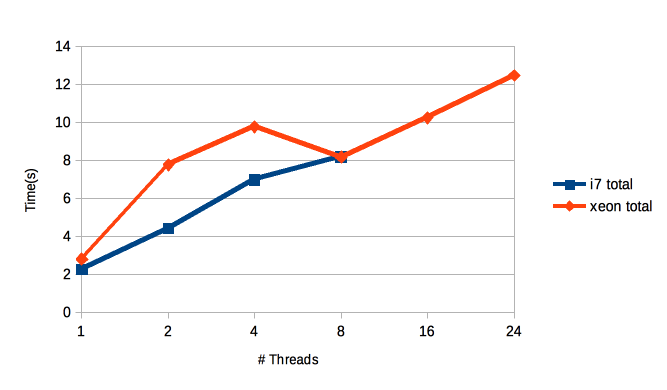
\includegraphics[width=\columnwidth]{../images/time_final.png}        
    \end{figure}

    As can be seen in the plot above, like our first OpenMP version, it still doesn't scale. This because the problems from bad data locality, are still there.

    \begin{figure}[H]
        \centering  
        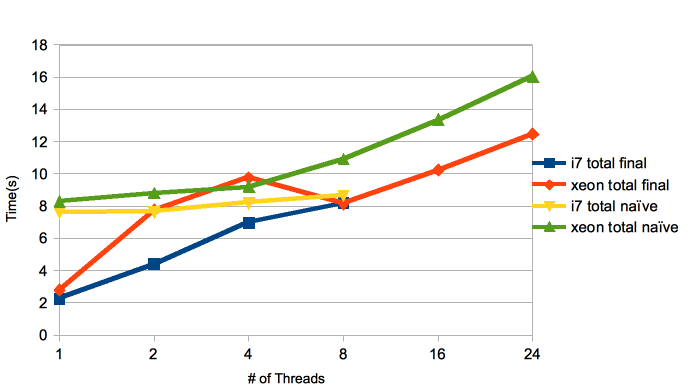
\includegraphics[width=\columnwidth]{../images/time_compare2.png}        
    \end{figure}

    However, by converting to SOA, the overall execution time was greatly reduced.

    \begin{figure}[H]
        \centering   
        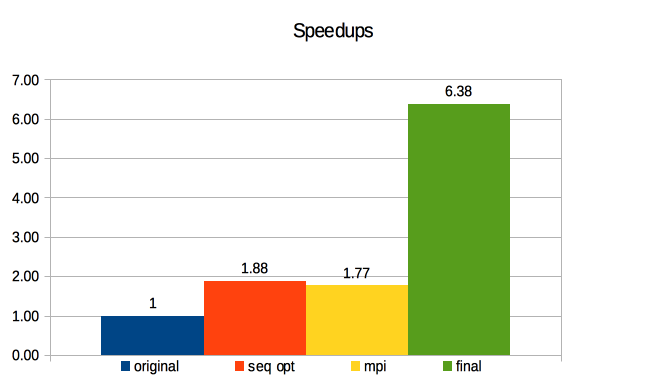
\includegraphics[width=\columnwidth]{../images/time_compared.png}        
    \end{figure}

    The figure above shows the speedups for the sequential versions of all implementations. As it can be seen, our SOA implementation has the best results. To improve the scalability, maybe the use of a mesh partitioning library, like parmetis, would help boost the performance, since that's the main problem with \emph{conv-diff}.


\section{Concluding Remarks}
\label{conc}

Conv-diff proved to be a problematic application, since our best efforts could not yield good results from any parallelization techniques. That being said, however, some improvements were made to the sequential version, especially in SOA implementation. \\
To fully take advantage of parallelization techniques, conv-diff needs a better structure for the mesh. However, to achieve this, we would more time around the source code. \\

\end{document}
